\documentclass[9pt,twocolumn,twoside]{pnas-new}
% Use the lineno option to display guide line numbers if required.

%%%%% NEW MATH DEFINITIONS %%%%%
\usepackage{amsmath,bbm,bm}
\usepackage{amssymb}
\usepackage{amsfonts}
\usepackage{amsthm}
\usepackage{mathtools}

% commands
% global count (no section number)
\newtheorem{thm}{Theorem}%[section]
\newtheorem{lem}{Lemma}
\newtheorem{prop}{Proposition}
\newtheorem{cor}{Corollary}
\newtheorem{conj}{Conjecture}
\newtheorem{aspt}{Assumption}
\newtheorem{claim}{Claim}
\newtheorem{rmk}{Remark}
\newtheorem{commt}{Comment}
\newtheorem{defn}{Definition}

% algorithm
%\usepackage{algorithm, algorithmic}
%\usepackage{algorithm2e}
\usepackage{tabularx}
%\usepackage[table,xcdraw]{xcolor}

% Comments
% \usepackage{xcolor} % already loaded
\newcount\comments  % 0 suppresses notes to selves in text
\comments=1  % TODO: change to 0 for final version
\newcommand{\genComment}[2]{\ifnum\comments=1{\textcolor{#1}{\textsf{\footnotesize #2}}}\fi}
\newcommand{\ed}[1]{\genComment{red}{[EI:#1]}}
\newcommand{\giles}[1]{\genComment{green}{[GH:#1]}}
\newcommand{\kevin}[1]{\genComment{blue}{[KT:#1]}}


% Mark sections of captions for referring to divisions of figures
\newcommand{\figleft}{{\em (Left)}}
\newcommand{\figcenter}{{\em (Center)}}
\newcommand{\figright}{{\em (Right)}}
\newcommand{\figtop}{{\em (Top)}}
\newcommand{\figbottom}{{\em (Bottom)}}
\newcommand{\captiona}{{\em (a)}}
\newcommand{\captionb}{{\em (b)}}
\newcommand{\captionc}{{\em (c)}}
\newcommand{\captiond}{{\em (d)}}


\newcommand\seq[2]{{#1}\!:\!{#2}}
\newcommand\R{\mathbb{R}}
\newcommand\Var{\mathrm{Var}}
\newcommand\var{\Var}
\newcommand\Cov{\mathrm{Cov}}
\newcommand\cov{\Cov}
\newcommand\iid{\mathrm{iid}}
\newcommand\dist{d}
\newcommand\lik{\mathcal{L}}
\newcommand\prob{\mathbb{P}}
\newcommand\E{\mathbb{E}}
\newcommand\loglik{\ell}
\newcommand\process{\texttt{process}}
\newcommand\dimtheta{\mathrm{dim}_{\Theta}}
\newcommand\param{\,;}
\newcommand\giventh\param
\newcommand\given{{\,\vert\,}}
\newcommand\code[1]{\texttt{#1}}
\newcommand\ceil[1]{\lceil #1 \rceil}
\newcommand\floor[1]{\lfloor #1 \rfloor}
\newcommand\1{\bm{1}}


% Highlight a newly defined term
\newcommand{\newterm}[1]{{\bf #1}}


% Figure reference, lower-case.
\def\figref#1{figure~\ref{#1}}
% Figure reference, capital. For start of sentence
\def\Figref#1{Figure~\ref{#1}}
\def\twofigref#1#2{figures \ref{#1} and \ref{#2}}
\def\quadfigref#1#2#3#4{figures \ref{#1}, \ref{#2}, \ref{#3} and \ref{#4}}
% Section reference, lower-case.
\def\secref#1{section~\ref{#1}}
% Section reference, capital.
\def\Secref#1{Section~\ref{#1}}
% Reference to two sections.
\def\twosecrefs#1#2{sections \ref{#1} and \ref{#2}}
% Reference to three sections.
\def\secrefs#1#2#3{sections \ref{#1}, \ref{#2} and \ref{#3}}
% Reference to an equation, lower-case.
\def\eqref#1{equation~\ref{#1}}
% Reference to an equation, upper case
\def\Eqref#1{Equation~\ref{#1}}
% A raw reference to an equation---avoid using if possible
\def\plaineqref#1{\ref{#1}}
% Reference to a chapter, lower-case.
\def\chapref#1{chapter~\ref{#1}}
% Reference to an equation, upper case.
\def\Chapref#1{Chapter~\ref{#1}}
% Reference to a range of chapters
\def\rangechapref#1#2{chapters\ref{#1}--\ref{#2}}
% % Reference to an algorithm, lower-case.
% \def\algref#1{algorithm~\ref{#1}}
% % Reference to an algorithm, upper case.
% \def\Algref#1{Algorithm~\ref{#1}}
% \def\twoalgref#1#2{algorithms \ref{#1} and \ref{#2}}
% \def\Twoalgref#1#2{Algorithms \ref{#1} and \ref{#2}}
% Reference to a part, lower case
\def\partref#1{part~\ref{#1}}
% Reference to a part, upper case
\def\Partref#1{Part~\ref{#1}}
\def\twopartref#1#2{parts \ref{#1} and \ref{#2}}

\def\eps{{\epsilon}}

\def\gN{{\mathcal{N}}}
\def\gX{{\mathcal{X}}}
\def\gY{{\mathcal{Y}}}


\makeatletter
\newcommand*{\addFileDependency}[1]{% argument=file name and extension
\typeout{(#1)}% latexmk will find this if $recorder=0
% however, in that case, it will ignore #1 if it is a .aux or 
% .pdf file etc and it exists! If it doesn't exist, it will appear 
% in the list of dependents regardless)
%
% Write the following if you want it to appear in \listfiles 
% --- although not really necessary and latexmk doesn't use this
%
\@addtofilelist{#1}
%
% latexmk will find this message if #1 doesn't exist (yet)
\IfFileExists{#1}{}{\typeout{No file #1.}}
}\makeatother

\newcommand*{\myexternaldocument}[1]{%
\externaldocument{#1}%
\addFileDependency{#1.tex}%
\addFileDependency{#1.aux}%
}

\templatetype{pnasresearcharticle} % Choose template
% {pnasresearcharticle} = Template for a two-column research article
% {pnasmathematics} %= Template for a one-column mathematics article
% {pnasinvited} %= Template for a PNAS invited submission

\begin{document}


\title{Inference for Dynamic and Latent Variable Models via Plug-and-Play Automatically Differentiable Particle Filtering}

% Use letters for affiliations, numbers to show equal authorship (if applicable) and to indicate the corresponding author
\author[a]{Kevin Tan}
\author[b,1]{Edward L. Ionides}
%\author[a]{Author Three}

\affil[a]{University of Pennsylvania}
\affil[b]{University of Michigan}
%\affil[c]{Affiliation Three}

% Please give the surname of the lead author for the running footer
\leadauthor{Tan}

% Please add a significance statement to explain the relevance of your work
\significancestatement{Many scientific models involve highly nonlinear stochastic dynamical systems, sometimes with noisy and incomplete measurements. Under the Markov assumption on system dynamics, previous work has provided methods of performing inference for these models. In particular, prior to this work, iterated filtering algorithms were the only class of algorithms for maximum likelihood estimation that did not require access to the system's transition probabilities, instead needing only a simulator of the system dynamics. We leverage recent advances in automatic differentiation to propose a hybrid algorithm that requires only a differentiable simulator for maximum likelihood estimation. Our new method dramatically outperforms previous approaches on a challenging problem in epidemiology.}

% Please include corresponding author, author contribution and author declaration information
\authorcontributions{Please provide details of author contributions here.}
\authordeclaration{Please declare any competing interests here.}
%\equalauthors{\textsuperscript{1}A.O.(Author One) contributed equally to this work with A.T. (Author Two) (remove if not applicable).}
\correspondingauthor{\textsuperscript{1}To whom correspondence should be addressed. E-mail: ionides@umich.edu}

% At least three keywords are required at submission. Please provide three to five keywords, separated by the pipe symbol.
\keywords{Sequential Monte Carlo $|$ Automatic Differentiation $|$ Particle Filter $|$ Markov Process $|$ Maximum Likelihood}

\begin{abstract}
\end{abstract}

\dates{This manuscript was compiled on \today}
\doi{\url{www.pnas.org/cgi/doi/10.1073/pnas.XXXXXXXXXX}}


\maketitle
\thispagestyle{firststyle}
\ifthenelse{\boolean{shortarticle}}{\ifthenelse{\boolean{singlecolumn}}{\abscontentformatted}{\abscontent}}{}

\firstpage{10}
% Use \firstpage to indicate which paragraph and line will start the second page and subsequent formatting. In this example, there are a total of 11 paragraphs on the first page, counting the first level heading as a paragraph. The value {12} represents the number of the paragraph starting the second page. If a paragraph runs over onto the second page, include a bracket with the paragraph line number starting the second page, followed by the paragraph number in curly brackets, e.g. "\firstpage[4]{11}".


% If your first paragraph (i.e. with the \dropcap) contains a list environment (quote, quotation, theorem, definition, enumerate, itemize...), the line after the list may have some extra indentation. If this is the case, add \parshape=0 to the end of the list environment.
\dropcap{M}any approaches to inference in highly nonlinear stochastic dynamical systems assume access to the probability density of next states given the current state.

This is a problem in some critical applications, such as disease modeling, where the models are complex enough that obtaining the density is intractable. However, the particle filter, a popular method for solving the filtering problem in partially-observed dynamical systems, does not require evaluation of the transition density of the latent Markov process, enabling an arbitrary model simulator to be plugged into the algorithm in a feature known as the plug-and-play property. 

Still, maximum likelihood parameter estimation can be challenging, especially when the Monte Carlo variance of the evaluation is high and the number of parameters is not small. Existing methods like the improved iterated filtering algorithm of Ionides et. al. \cite{Ionides_infpomp} converge quickly to a neighborhood of the MLE, but struggle to optimize the last few units of log-likelihood. 

\kevin{TODO: (1) Fix beta smoothness to d(n) at no more than O(n), (2) add story to say that no one spotted that it could have been plug-and-play because of e.g. reasons why they would stumble, (3) }

\kevin{Previous literature: Doucet waymo only applicable to policy plus deterministic dynamics}


We propose a hybrid algorithm that u

Unlike IF2, we explicitly characterize our method's rate of convergence

% IF2 is SGD that iterates through the data sequentially in the 1:N sense, and noisy/mini-batch GD in the 1:J sense. 
% ADPF is batch GD in the 1:N sense, and noisy/mini-batch GD in the 1:J sense. 


Algorithmic differentiation potentially facilitates numerical optimization, but currently its use for particle filters is limited. We investigate ways to use algorithmic differentiation of particle filters within the confines of the plug-and-play property, with the goal of enhancing current inference capabilities for general POMP models.


\textbf{The issue:} Particle filters provide convenient approaches to evaluating the log-likelihood function for partially observed Markov process (POMP) models. However, using this evaluator to obtain a maximum likelihood parameter estimate can be challenging -- especially when the Monte Carlo variance of the evaluation is high and the number of parameters is not small. Empirically, methods such as the improved iterated filtering algorithm (IF2) from Ionides et. al. \cite{Ionides_infpomp} rapidly converge to a neighborhood of the optimum but struggle at finding the exact optimum due to Monte Carlo variance, even with an annealing random walk standard deviation. 

A potential solution to this could lie in auto-differentiation (AD). This would allow for the use of first and second-order iterative optimization techniques. However, though AD could potentially facilitate numerical optimization, its use for plug-and-play particle filters has so far been limited. This is potentially because particle filtering methods are inherently non-differentiable due to the resampling step that may take place in between iterations. 

\subsection*{The importance of the plug-and-play property:} Performing inference in highly nonlinear stochastic dynamical systems is a challenging problem. Although many methods for inference assume access to the density of state transitions, this is often not available, especially in critical applications like epidemiology.

Basic particle filtering algorithms do not require evaluation of the transition density of the latent Markov process, in a feature known as the \textbf{plug-and-play property} \cite{Breto_timeseriesmech} since it enables an arbitrary model simulator to be plugged into the algorithm. We investigate ways to use algorithmic differentiation of particle filters within the confines of the plug-and-play property, with the goal of enhancing current inference capabilities for general POMP models.

\subsection*{Other potential applications:} This has applications beyond the obvious one of learning model parameters via first or second-order optimization routines. For example, it could be a step towards developing very general Hamiltonian Monte Carlo methods for particle MCMC, as Rosato et. al. \cite{rosato22b} do by using previous work such as \cite{scibior2021dpf, doucet2011sf} (and we conjecture that the seed-fixing derivatives of Rosato et. al. are the same as these as an immediate consequence of section \ref{subsec:scibiorrel}) to differentiate the particle filter. 

\section*{Guide to using this template on Overleaf}

Please note that whilst this template provides a preview of the typeset manuscript for submission, to help in this preparation, it will not necessarily be the final publication layout. For more detailed information please see the \href{https://www.pnas.org/page/authors/format}{PNAS Information for Authors}.

If you have a question while using this template on Overleaf, please use the help menu (``?'') on the top bar to search for \href{https://www.overleaf.com/help}{help and tutorials}. You can also \href{https://www.overleaf.com/contact}{contact the Overleaf support team} at any time with specific questions about your manuscript or feedback on the template.

\subsection*{Author Affiliations}

Include department, institution, and complete address, with the ZIP/postal code, for each author. Use lower case letters to match authors with institutions, as shown in the example. PNAS strongly encourages authors to supply an \href{https://orcid.org/}{ORCID identifier} for each author. Individual authors must link their ORCID account to their PNAS account at \href{http://www.pnascentral.org/}{www.pnascentral.org}. For proper authentication, authors must provide their ORCID at submission and are not permitted to add ORCIDs on proofs.

\subsection*{Submitting Manuscripts}

All authors must submit their articles at \href{http://www.pnascentral.org/cgi-bin/main.plex}{PNAScentral}. If you are using Overleaf to write your article, you can use the ``Submit to PNAS'' option in the top bar of the editor window.

\subsection*{Format}

Many authors find it useful to organize their manuscripts with the following order of sections: title, author line and affiliations, keywords, abstract, significance statement, introduction, results, discussion, materials and methods, acknowledgments, and references. Other orders and headings are permitted.

\subsection*{Manuscript Length}

A standard 6-page article is approximately 4,000 words, 50 references, and 4 medium-size graphical elements (i.e., figures and tables). The preferred length of articles remains at 6 pages, but PNAS will allow articles up to a maximum of 12 pages.

\subsection*{References}

References should be cited in numerical order as they appear in text; this will be done automatically via bibtex, e.g. \cite{belkin2002using} and \cite{berard1994embedding,coifman2005geometric,phdthesis,masterthesis}. All references cited in the main text should be included in the main manuscript file.

\subsection*{Data Archival}

PNAS must be able to archive the data essential to a published article. Where such archiving is not possible, deposition of data in public databases, such as GenBank, ArrayExpress, Protein Data Bank, Unidata, and others outlined in the \href{https://www.pnas.org/author-center/editorial-and-journal-policies#materials-and-data-availability}{Information for Authors}, is acceptable.

\subsection*{Language-Editing Services}
Prior to submission, authors who believe their manuscripts would benefit from professional editing are encouraged to use a language-editing service (see list at https://www.pnas.org/author-center/language-editing). PNAS does not take responsibility for or endorse these services, and their use has no bearing on acceptance of a manuscript for publication.

\begin{figure}%[tbhp]
\centering
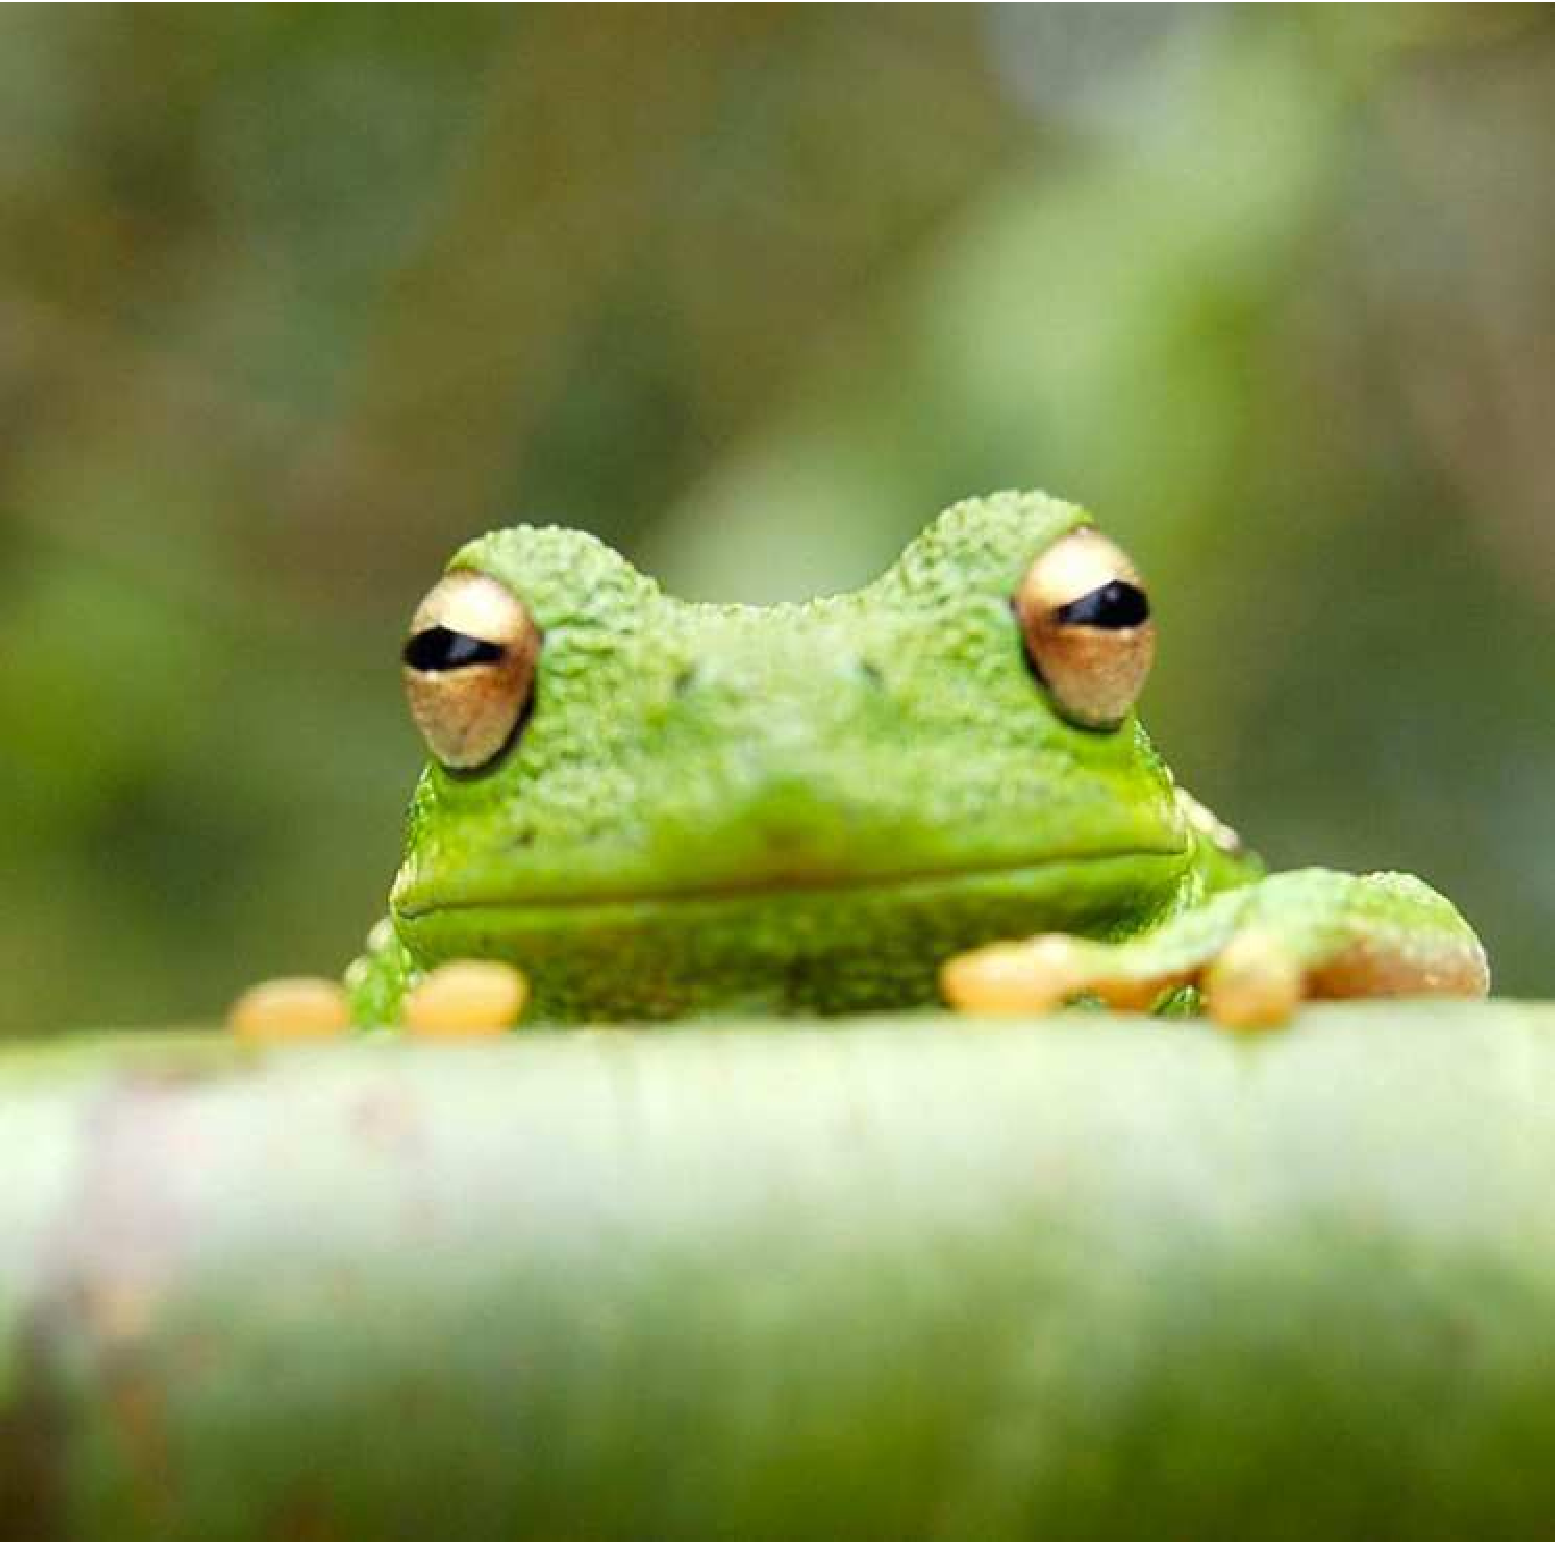
\includegraphics[width=.8\linewidth]{frog.pdf}
\caption{Placeholder image of a frog with a long example legend to show justification setting.}
\label{fig:frog}
\end{figure}



\begin{table}[t!]
\centering
\caption{Comparison of the fitted potential energy surfaces and ab initio benchmark electronic energy calculations}
\begin{tabular}{lrrr}
Species & CBS & CV & G3 \\
\midrule
1. Acetaldehyde & 0.0 & 0.0 & 0.0 \\
2. Vinyl alcohol & 9.1 & 9.6 & 13.5 \\
3. Hydroxyethylidene & 50.8 & 51.2 & 54.0\\
\bottomrule
\end{tabular}

\addtabletext{nomenclature for the TSs refers to the numbered species in the table.}
\end{table}


\subsection*{Digital Figures}

EPS, high-resolution PDF, and PowerPoint are preferred formats for figures that will be used in the main manuscript. Authors may submit PRC or U3D files for 3D images; these must be accompanied by 2D representations in TIFF, EPS, or high-resolution PDF format. Color images must be in RGB (red, green, blue) mode. Include the font files for any text.

Images must be provided at final size, preferably 1 column width (8.7cm). Figures wider than 1 column should be sized to 11.4cm or 17.8cm wide. Numbers, letters, and symbols should be no smaller than 6 points (2mm) and no larger than 12 points (6mm) after reduction and must be consistent.

Figures and tables should be labelled and referenced in the standard way using the \verb|\label{}| and \verb|\ref{}| commands.

Figure \ref{fig:frog} shows an example of how to insert a column-wide figure. To insert a figure wider than one column, please use the \verb|\begin{figure*}...\end{figure*}| environment. Figures wider than one column should be sized to 11.4 cm or 17.8 cm wide. Use \verb|\begin{SCfigure*}...\end{SCfigure*}| for a wide figure with side legends.

\begin{SCfigure*}[\sidecaptionrelwidth][t!]
\centering
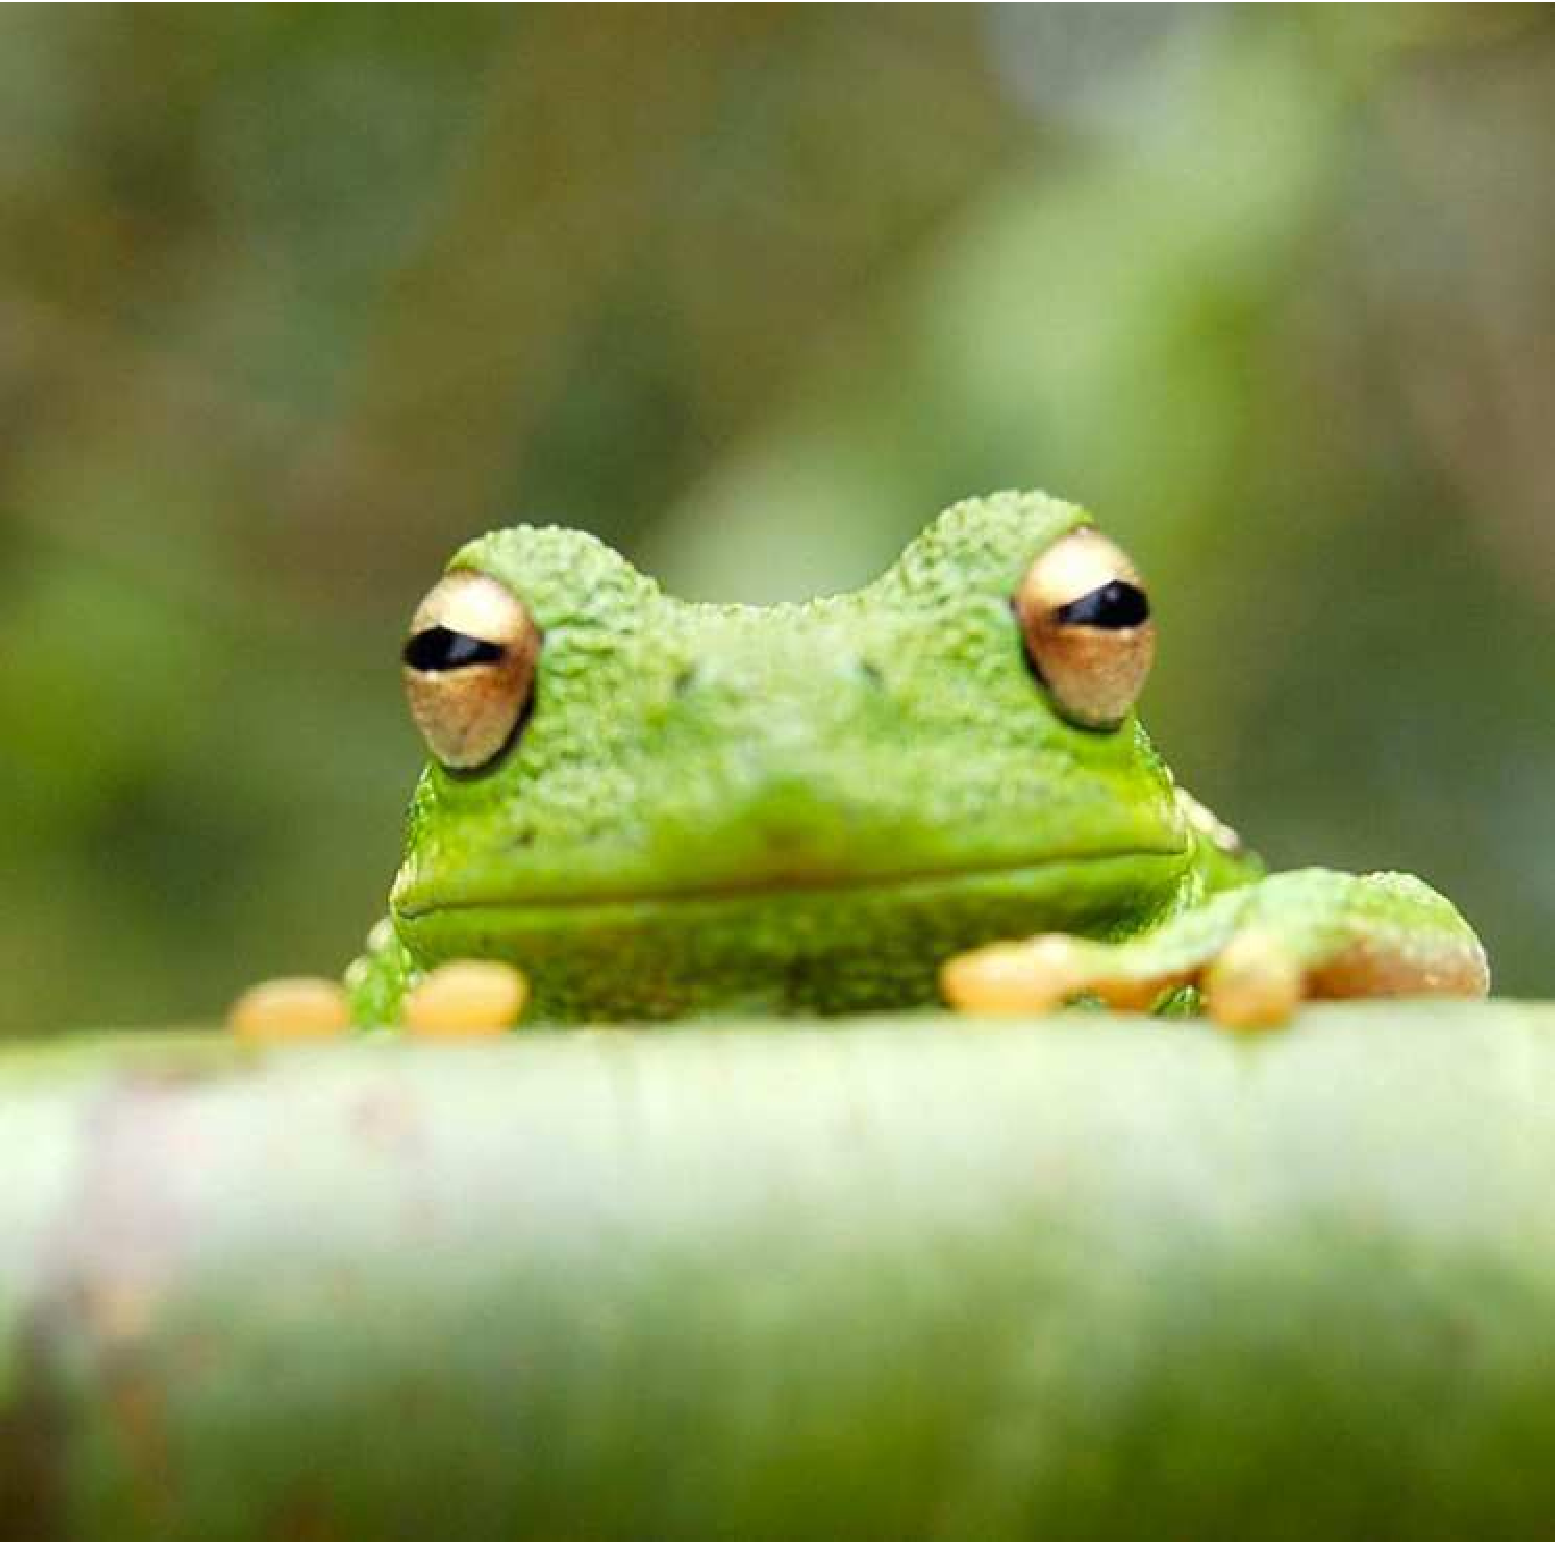
\includegraphics[width=11.4cm,height=11.4cm]{frog.pdf}
\caption{This legend would be placed at the side of the figure, rather than below it.}\label{fig:side}
\end{SCfigure*}


\subsection*{Tables}
Tables should be included in the main manuscript file and should not be uploaded separately.


\subsection*{Single column equations}

Authors may use 1- or 2-column equations in their article, according to their preference.

To allow an equation to span both columns, use the \verb|\begin{figure*}...\end{figure*}| environment mentioned above for figures.

Note that the use of the \verb|widetext| environment for equations is not recommended, and should not be used.

\begin{figure*}[bt!]
\begin{align*}
(x+y)^3&=(x+y)(x+y)^2\\
       &=(x+y)(x^2+2xy+y^2) \numberthis \label{eqn:example} \\
       &=x^3+3x^2y+3xy^3+x^3.
\end{align*}
\end{figure*}



\subsection*{Supporting Information Appendix (SI)}

Authors should submit SI as a single separate SI Appendix PDF file, combining all text, figures, tables, movie legends, and SI references. SI will be published as provided by the authors; it will not be edited or composed. Additional details can be found in the \href{https://www.pnas.org/authors/submitting-your-manuscript#manuscript-formatting-guidelines}{PNAS Author Center}. The PNAS Overleaf SI template can be found \href{https://www.overleaf.com/latex/templates/pnas-template-for-supplementary-information/wqfsfqwyjtsd}{here}. Refer to the SI Appendix in the manuscript at an appropriate point in the text. Number supporting figures and tables starting with S1, S2, etc.

Authors who place detailed materials and methods in an SI Appendix must provide sufficient detail in the main text methods to enable a reader to follow the logic of the procedures and results and also must reference the SI methods. If a paper is fundamentally a study of a new method or technique, then the methods must be described completely in the main text.

\subsubsection*{SI Datasets}

Supply .xlsx, .csv, .txt, .rtf, or .pdf files. This file type will be published in raw format and will not be edited or composed.


\subsubsection*{SI Movies}

Supply Audio Video Interleave (avi), Quicktime (mov), Windows Media (wmv), animated GIF (gif), or MPEG files. Movie legends should be included in the SI Appendix file. All movies should be submitted at the desired reproduction size and length. Movies should be no more than 10MB in size.




\matmethods{Please describe your materials and methods here. This can be more than one paragraph, and may contain subsections and equations as required.

\subsection*{Subsection for Method}
Example text for subsection.
}

\showmatmethods{} % Display the Materials and Methods section

\acknow{Please include your acknowledgments here, set in a single paragraph. Please do not include any acknowledgments in the Supporting Information, or anywhere else in the manuscript.}

\showacknow{} % Display the acknowledgments section


\bibsplit[2]
%Use \bibsplit to split the references from the body of the text. Value "[2]" represents the number of reference in the left column (Note: Please avoid single column figures & tables on this page.)

% Bibliography
\bibliography{pnas-sample}

\end{document}
